\documentclass{../local}
\begin{document}
Dit project is gestart vanuit een nieuw concept. Om dit concept mogelijk te maken moet er gebruik gemaakt worden van meerdere componenten. Om een weloverwogen keuze te maken wordt in dit hoofdstuk de keuze gemaakt van de volgende componenten en beargumenteerd waarom die keuze is gemaakt:
\begin{itemize}
\item Keuze van benodigde software aan de hand van de requirements
\item Keuze van hardware die geschikt is voor de gekozen software met in acht neming van de gekozen software

\end{itemize}

\section{Software Keuze}
Voor Wireless Sensor Networks zijn vele software pakketten beschikbaar. In deze sectie zullen meerdere met elkaar worden vergeleken en de beste gekozen. Om zeker te zijn dat het mogelijk is om er makkelijk mee te werken, wordt er alleen gekeken naar de populairdere oplossingen. Dat betekent dat het pakket programmeer voorbeelden moet hebben, in de laatste 2 jaren aan moet zijn ontwikkeld, of geplande verbeteringen, en het bekend is dat er door andere partijen actief gebruik van wordt gemaakt.

\begin{wrapfigure}[15]{r}{0.55\textwidth}
	\vspace{-15pt}
	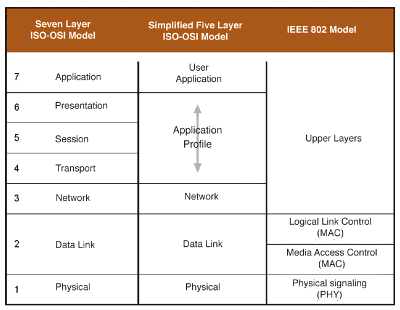
\includegraphics[width=9cm]{../images/OSI-IEE802}
	\caption{\emph{OSI model IEEE 802.15.4 \cite{gutierrez2004low}}} \label{fig:OSIIEEE}

\end{wrapfigure}

De volgende pakketten worden bestudeerd: ZigBee, Z-Wave, TinyOS, ContikiOS en RIOT. Voor elk onderdeel wordt beschreven hoe het systeem werkt en daarna de voordelen en nadelen uiteen gezet. Als laatste wordt de gemaakte keuze beschreven.

\subsection{ZigBee}

ZigBee is een standaard bedoeld voor low-cost, energiezuinige draadloze 'mesh'- of 'ster' netwerken. Een mesh netwerk maakt het mogelijk om een hoge robuustheid te garanderen en groot netwerk op te bouwen. Deze netwerken kunnen theoretisch tot ongeveer 65.000 nodes bestaan. Zigbee huisvest ook routing technieken en beveiliging binnen de netwerken. Ontwikkelaars die ZigBee gebruiken of de ZigBee standaard verbeteren zitten binnen de ZigBee Alliance, wel te vergelijken als de WiFi Alliance.

Een zigbee netwerk bestaat uit 3 componenten: één ZigBee Coordinator, ZigBee Routers en ZigBee End Devices. De Coordinator is de maker van het netwerk en bepaalt de netwerk instellingen en beveiliging. Routers zijn bedoeld om het netwerk te vergroten en berichten door te sturen. End Devices zijn randapparaten die de omgeving meten of controleren.

ZigBee is gebouwd op de IEEE standaard 802.15.4. Deze standaard beschrijft de fysieke laag en de data-link laag van het OSI model te zien in in de rechter kolom van figuur \ref{fig:OSIIEEE}. De fysieke laag van het OSI model bepaalt hoe data draadloos wordt verzonden (modulering) en in welke radioband. De Data-Link laag beschrijft controle mechanismes hoe en wanneer een module binnen een IEEE 802.15.4 netwerk mag verzenden. De overdrachtsnelheid hierbij is 250 kb/s bij gebruik van het 2.4GHz spectrum wat wereldwijd beschikbaar is.

De opvolgende lagen van het OSI model zijn ingevuld door de ZigBee standaard. ZigBee volgt het versimpelde vijf lagen OSI model te zien in figuur \ref{fig:OSIIEEE}. ZigBee biedt applicatie profielen aan die functionaliteiten bieden voor bepaalde gebieden zoals: Home Automation, Snart Energy of Building Automation. Bovenop deze profielen kan de benodigde applicatie gebouwd worden.\footnote{\url{http://www.zigbee.org/}}

\subsubsection{Voordelen/Nadelen}

ZigBee is veelgebruikt en er zijn vele bedrijven die oplossingen aanbieden. Ook zijn er veel programmeer voorbeelden beschikbaar via verschillende leveranciers zoals Texes Instruments en Libelium. Het gebruik van de Zigbee profielen versimpelt de ontwikkeling van applicaties aanzienlijk.

Bekend met ZigBee is dat het netwerk gedeelte onveranderbaar is. Er kan een netwerk topologie gekozen worden waar dan niet van kan worden afgeweken. Wel alle belangrijke soorten topologieën zijn beschikbaar.

Het netwerk van ZigBee werkt met een centrale Coordinator die zaken als routing en veiligheid verzorgen. In de oudere ZigBee standaard (2006) resulteerde het falen van de coordinator tot het falen van het netwerk. Dit is in nieuwere versies opgelost door de optie te bieden om binding tables van een netwerk te distribueren over het gehele netwerk.

Hoewel dit een verbetering is, geeft het niet de flexibiliteit en robuustheid voor End Devices. End Devices die als nieuw of opnieuw het netwerk moeten betreden of kunnen dat niet meer wanneer de coordinator is uitgevallen. Dit is niet praktisch bij een veiligheidsinstallatie voor branddetectie. Nodes (of Devices in het geval van ZigBee) binnen een netwerk kunnen bij brand of andere situatie uitvallen. Een ZigBee netwerk kan hiermee slecht omgaan.

%ik bedoel hier dat de specificaties van zigbee niet zomaar beschikbaar zijn...
Het is ook niet direct mogelijk om de netwerklaag van ZigBee naar wens aan te passen. Hiervoor is het nodig om lid te zijn van de ZigBee Alliance, wat op moment van schrijven vanaf \$4.000 per jaar kost\footnote{\url{http://www.zigbee.org/Join/MembershipForms.aspx}}. Dit is ook het geval als een bedrijf ZigBee gecertificeerde producten wil verkopen.

\subsection{Z-Wave}
Z-Wave is een gepattenteerde draadloze standaard ontwikkeld door Zensys en eigendom van Sigma Designs. Deze standaard is niet open voor iedereen, maar alleen voor klanten voor het bedrijf zelf. De Z-Wave fysieke en MAC lagen zijn inbegrepen in de G.9959 standaard van de International Telecommunications Union (ITU)\cite{ITUG9959}.

Z-Wave werkt in de sub-1-GHz radio frequenties. Elk Z-Wave netwerk beschikt over een master controller die het netwerk beheert. Een netwerk kan over maximaal 232 nodes beschikken en kan worden uitgebreid door meerdere netwerken met master controllers op te zetten en die te koppelen.

Chips zijn alleen te koop bij Sigma Designs, maar verkopen alleen bij grote afnemers. Er zijn meerdere bedrijven die Z-Wave producten verkopen. Deze producten zijn vooral gericht op Home Automation (b.v. Afstandbestuurbare lampen, deursloten en thermostaten).

\subsubsection{Voordelen/Nadelen}
Z-Wave is voornamelijk gericht op de Home Automation markt. Hierdoor is het mogelijk dat door deze focus Z-Wave niet toepasbaar is op dit project. In de praktijk is het namelijk zo dat een netwerk ongeveer 10 nodes ondersteunt \cite{ednZWave}.

De licenties gekoppeld aan deze technologie maakt de drempel tot gebruik ook hoog. Een development kit kost \$3.000 om te kunnen werken met de standaard. Het product (wat Z-Wave gebruikt) moet eerst getest worden door Sigma Designs, waarna het legaal op de markt gezet mag worden.

Z-Wave moet ook volgens de certificering koppelbaar zijn met andere Z-Wave apparaten. Dit kan een veiligheidssysteem in gevaar brengen doordat andere producten te veel invloed hebben op het netwerk.

\subsection{TinyOS}
TinyOS is een embedded operating system ontworpen voor low-power wireless sensor netwerken. Het is een open-source project en uitgebracht volgens het BSD-licentie\footnote{\url{http://opensource.org/licenses/BSD-3-Clause}}. Versie 1 van TinyOS is in 2002 uitgebracht tot aan versie 2.1.2 in augustus 2012. Het OS is nog steeds actief met ontwikkelingen.

Applicaties die op TinyOS draaien worden geprogrammeerd in nesC\cite{nesC}. NesC is een uitbreiding op de C programmeertaal. NesC voegt mechanismen toe zodat applicaties als componenten worden geprogrammeerd.

TinyOS is een op events gebaseerde non-blocking OS. Het heeft een non-preemptive scheduler en taken worden volgens de First In First Out volgorde uitgevoerd. Er is één stack beschikbaar voor alle taken binnen het systeem, wat zorgt voor weinig RAM verbruik. Verder heeft TinyOS hardware abstractie lagen, zodat ontwikkelaars makkelijker sensoren kunnen gebruiken.

Voor netwerk mogelijkheden heeft TinyOS een uitgebreide set aan componenten. Voor energiebesparing van de radio component zijn er werkcycli gedefinieerd, zo zal de radio niet continu aanstaan en stroom verbruiken.

% - nieuwe programmeertaal NESC

% + 6LoWPAN

\subsection{ContikiOS}
%vrije RIME protocol. compatible met 802.15.4 frames
%simpele driver development
%switchen van mac protocol / RDC protocol...maken van dit soort componenten is relatief simpel( mac / rdc ).
%++++++SIMULATIE
\subsection{RIOT}


\section{Hardware}
Met gebruik van de gekozen wireless transmissie techniek, software en de requirements kan de hardware gekozen worden. 
%

\end{document}